\section{Beispeilhafte Prozesse auf dem Werksgelände}\label{sec:realeIst}
Dieser Anhang befasst sich mit der Kommunikation und den einzelnen Schritten bei der Verladung der zugehörigen Parteien. Die hier abgebildeten Prozesse entsprechen der Abwicklung auf dem Betriebsgelände seitens der IDR (Industrieterrains Düsseldorf-Reisholz AG) und stammen aus einem Gespräch mit dem Eisenbahnbetriebsleiter.\cite{IDR} Die IDR verfährt für verschiedenen Kunden volle und leere Kesselwagen unteranderem auch mit Gefahrgut, sowie Schüttgutwagen. \par
Auf dem Betriebsgelände werden die Wagen, auch wenn sie später als Ganzzug das Werk verlassen wie Einzelwagen oder kleine Wagengruppen behandelt. Besonderer Augenmerk wird auf die drei beteiligten Parteien 'Disposition', 'Verlader' und 'Lokrangierführer' gelegt. Da im Kapitel \ref{sec:Istzustand} bereits auf die Handgriffe des Lokrangeirführers eingegangen wurde, findet das hier nicht mehr ausführlich statt. Die Kupplungsvorgänge, technischen Wagenbehandlungen und Bremsproben entsprechen den bereits beschriebenen.

\subsection{Beschreibung des Prozesses}
Die beteiligten Parteien arbeiten, wie auf Abbildung \ref{fig:IDR_Warenausgang} zu sehen, Hand in Hand. Die Kommunikation findet über Datenverarbeitungssysteme (DVS), wie SAP, mündlich, beispielsweise telefonisch oder über Funk, oder auf Papier statt.\par
\begin{figure}
    \centering
    % Define block styles
\tikzstyle{block} = [rectangle, fill=blue!20, text width=5em, text centered, rounded corners, minimum height=4em, text width=8em]
\tikzstyle{cloud} = [draw, rectangle, fill=gray!20, node distance=2.5cm, minimum height=2em]
\tikzstyle{invisible} = [rectangle]


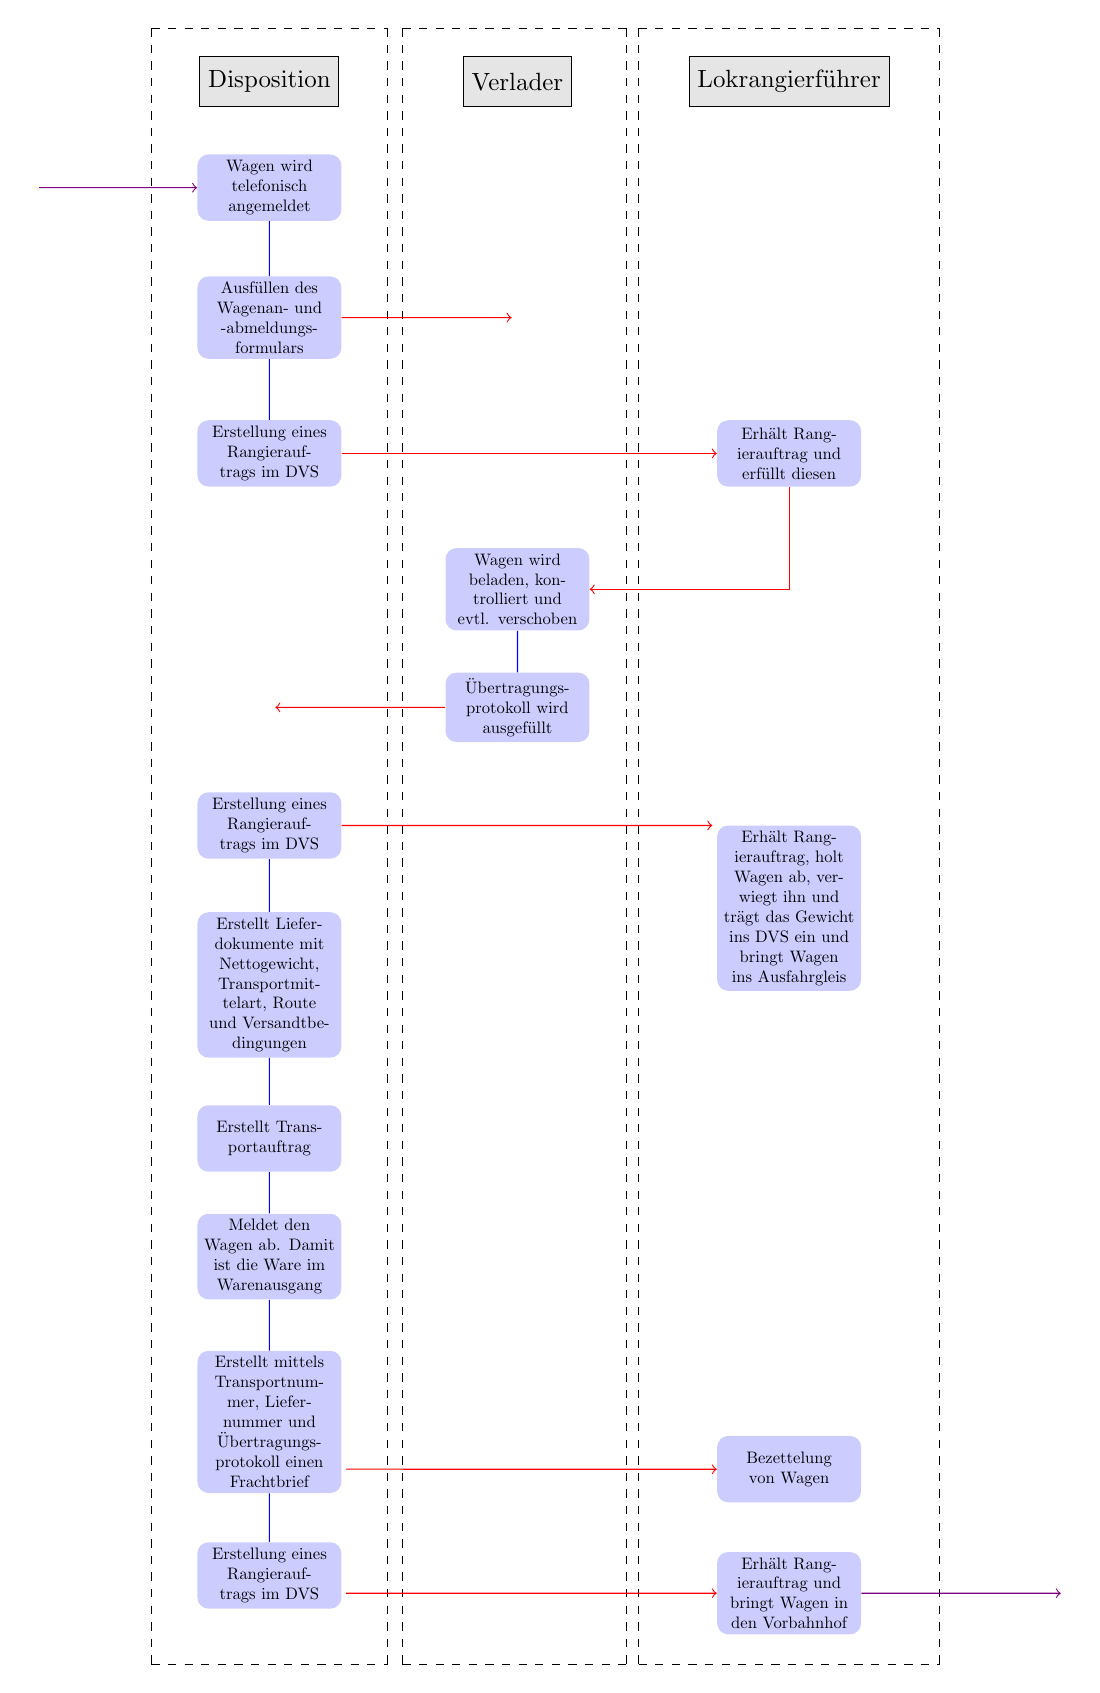
\begin{tikzpicture}[scale=0.75, every node/.style={scale=0.6}]
% Place nodes
    \node[invisible] at (-8, -1.5) (anmeldung) {};
    \node[cloud, scale=1.5] at (-4,0.3)      (dispo)         {Disposition};
    \node[cloud, scale=1.5] at (0.2, 0.3)      (verlader)      {Verlader} ;
    \node[cloud, scale=1.5] at (4.8,0.3)       (rangierende)   {Lokrangierführer};
        \node[invisible] at (-8, -1.5) (anmeldung) {};
    \node[block] at (-4, -1.5)  (Wagen)         {Wagen wird telefonisch angemeldet};
    \node[block] at (-4, -3.7)  (Waamf)         {Ausfüllen des Wagenan- und -abmeldungs- formulars};
        \node[invisible] at (0.2, -3.7) (vInfo) {};
    \node[block] at (-4, -6)    (RA)            {Erstellung eines Rangierauftrags im DVS};
    \node[block] at (4.8, -6)     (RA2)           {Erhält Rangierauftrag und erfüllt diesen};
    \node[block] at (0.2, -8.3)   (beladung)      {Wagen wird beladen, kontrolliert und evtl. verschoben};
    \node[block] at (0.2, -10.3)  (ueprot)        {Übertragungs- protokoll wird ausgefüllt};
        \node[invisible] at (-4, -10.3) (dInfo) {};
    \node[block] at (-4, -12.3) (RA3)           {Erstellung eines Rangierauftrags im DVS};
    \node[block] at (4.8, -13.7)  (RA4)           {Erhält Rangierauftrag, holt Wagen ab, verwiegt ihn und trägt das Gewicht ins DVS ein und bringt Wagen ins Ausfahrgleis};
    \node[block] at (-4, -15)   (Lieferdoc)     {Erstellt Lieferdokumente mit Nettogewicht, Transportmittelart, Route und Versandtbedingungen};
    \node[block] at (-4, -17.6) (Transportdoc)  {Erstellt Transportauftrag};
    \node[block] at (-4, -19.6) (abmelden)      {Meldet den Wagen ab. Damit ist die Ware im Warenausgang};
    \node[block] at (-4, -22.4) (Frachtbrief)   {Erstellt mittels Transportnummer, Liefernummer und Übertragungs- protokoll einen Frachtbrief};
    \node[block] at (4.8, -23.2)  (Zettel)        {Bezettelung von Wagen};
    \node[block] at (-4, -25.0) (RA5)           {Erstellung eines Rangierauftrags im DVS};
    \node[block] at (4.8, -25.3)  (RA6)           {Erhält Rangierauftrag und bringt Wagen in den Vorbahnhof};
        \node[invisible] at (9.5, -25.3) (ende) {};

% Draw edges
    %Kasten Dispo
    \draw[dashed] (-6, 1.2) -- (-6,-26.5);
    \draw[dashed] (-6, 1.2) -- (-2, 1.2);
    \draw[dashed] (-2, 1.2) -- (-2, -26.5);
    \draw[dashed] (-6, -26.5) -- (-2, -26.5);
    %Kasten Verlader
    \draw[dashed] (-1.75, 1.2) -- (2.05, 1.2);
    \draw[dashed] (-1.75, 1.2) -- (-1.75, -26.5);
    \draw[dashed] (-1.75, -26.5) -- (2.05, -26.5);
    \draw[dashed] (2.05, 1.2) -- (2.05, -26.5);
    %Kasten LRF
    \draw[dashed] (2.25, 1.2) -- (2.25, -26.5);
    \draw[dashed] (2.25, 1.2) -- (7.35, 1.2);
    \draw[dashed] (2.25, -26.5) -- (7.35, -26.5);
    \draw[dashed] (7.35, 1.2) -- (7.35, -26.5);
    
    %Pfeile ohne Beginn
    \draw[->, color=violet] (anmeldung) -- (Wagen);
    %Pfeile ohne Ende 
    \draw[->, color=red] (Waamf) -- (vInfo);
    \draw[->, color=red] (ueprot) -- (dInfo);
    \draw[->, color=violet] (RA6) -- (ende);
    %Pfeile mit Ende
    \draw[-, color=blue!100] (Wagen) -- (Waamf);
    \draw[-, color=blue] (Waamf) -- (RA);
    \draw[->, color=red] (RA) -- (RA2);
    \draw[->, color=red] (RA2) |- (beladung);
    \draw[-, color=blue] (beladung) -- (ueprot);
    \draw[->, color=red] (RA3) -- (3.5, -12.3);
    \draw[-, color=blue] (RA3) -- (Lieferdoc);
    \draw[-, color=blue] (Lieferdoc) -- (Transportdoc);
    \draw[-, color=blue] (Transportdoc) -- (abmelden);
    \draw[-, color=blue] (abmelden) -- (Frachtbrief);
    \draw[->, color=red] (-2.7, -23.2) -- (Zettel);
    \draw[-, color=blue] (Frachtbrief) -- (RA5);
    \draw[->, color=red] (-2.7, -25.3) -- (RA6);
    
\end{tikzpicture}

    \caption{Prozess der Verladung bei der IDR}
    \label{fig:IDR_Warenausgang}
\end{figure}
Der Wagen wird vom Vorbahnhof telefonisch bei der Disposition angemeldet. Diese füllt ein Wagenan- und -abmeldungsformular aus und leitet es schriftlich an den Verlader weiter. Danach wird ein Rangierauftrag im Datenverarbeitungssystem erstellt.\par
Diesen erhält der Lokrangierführer entweder mündlich (per Funk oder telefonisch) oder schriftlich und führt ihn aus.\par
Danach wird der oder die Wagen beladen und mittels Checkliste kontrolliert. Die Checkliste wird beim Verlader und am Güterwagen aufbewahrt. Je nach Rangierauftrag werden die Wagen dann vom Verlader verschoben und weitere Beladen oder abgestellt. Danach füllt der Verlader das Übertragungsprotokoll aus und leitet es an die Disposition weiter.\par
Die Disposition erstellt erneut einen Rangierauftrag im DVS und leitet diesen an den LrF weiter.\par
Der LrF erhält diesen Rangierauftrag, holt den oder die Wagen ab, verwiegt ihn und trägt das Gewicht ins DVS ein. Danach wird der Wagen oder der Wagenzug auf dem Ausfahrgleis abgestellt und mit eventuell anderen dort stehenden Wagen gekuppelt.\par
Währenddessen erstellt die Disposition die Lieferdokumente mit dem (Netto-)Gewicht, der Transportmittelart, der Route und den Versandbedingungen. Anschließend wird ein Transportauftrag erstellt, der Wagen abgemeldet und die Ware im Warenausgang vermerkt. Im Anschluss wird der Frachtbrief mit der Transportnummer, der Liefernummer und dem Übertragungsprotokoll erstellt.\par
Mit einer vereinfachten Variante des Frachtbriefes wird der Wagen vom LrF bezettelt.\par
Für die Ausfahrt des Wagenzugs in den Vorbahnhof, erstellt die Disposition wieder einen Rangierauftrag und teilt diesem dem LrF mit.\par
Der LrF rangiert die Wagen in den Vorbahnhof.\par
Im Vorbahnhof werden die Wagen dann mit einer Streckenlok gekoppelt und gehen in den geplanten Umlauf.

\subsection{Unterschiede in den Prozessen}
Der hier beschriebene Prozess des Warenausgangs von Kesselwagen unterscheidet sich selbstverständlich etwas von einem Wareneingang oder auch von Warenein- und -ausgängen von anderen Wagentypen und soll nur als Beispiel stehen. Ein paar Unterschiede werden in den folgenden Abschnitten näher beleuchtet.
\subsubsection{Wareneingang}
Wenn volle Wagen ankommen, werden diese sehr ähnlich verarbeitet.Der Wagen wird vorher verwogen und der Lieferschein mit dem Inhalt verglichen. Zusätzlich findet ein Vermerk des Wareneingangs statt. Des Weiteren erhält die Ladung eine Chargennummer zur Nachverfolgung.
\subsubsection{Fahrten am Wochenende}
Wagen können auch am Wochenende ohne Rangierauftrag ins Ladegleis geschoben werden. Montags wird dann die Abholung mittels Übertragung des Wagenan- und -abmeldungsformulars sowie des Übertragungsprotokoll nachgeholt.
\subsubsection{Gefahrgut}
Bei reaktionsreichem Ladegut (Gefahrgut) kann es sein, dass diese nur zu bestimmten Zeiten verschoben werden dürfen. Alternative Regelungen können sein,  dass sie nur alleine oder mit wenigen anderen Wagen verschoben oder abgestellt werden dürfen; oder auch dass nur eine bestimme Anzahl von Wagen auf dem Gelände oder in dem Bereich sein dürfen.
